\section{Einführung}

\notedate{01.03.2023}
Zu Beginn wird der Begriff einer allgemeinen (oder auch universellen) Algebra definiert und es werden weiter einige spezielle Algebren vorgestellt.

\begin{definition}\label{def:algebra}\label{def:allg_algebra}
    Seien $A$ eine beliebige Menge, $\tau = (n_i)_{i \in I}$ eine Familie aus $\mathbb{N}_0$ über einer beliebigen Indexmenge $I$ und $(f_i)_{i \in I}$ eine Familie von Funktionen, wobei $f_i: A^{n_i} \to A$ ist. 
    Das Tupel $\mathfrak{A} = (A, (f_i)_{i \in I})$ heißt dann \emph{(allgemeine) Algebra}\index{Algebra!allgemeine} vom \emph{Typ}\index{Algebra!Typ} $\tau$ oder auch \emph{$\tau$-Algebra}. Die einzelnen Funktionen $f_i$ nennt man \emph{fundamentale Operationen}\index{fundamentale Operation} und haben \emph{Stelligkeit}\index{Stelligkeit} oder auch \emph{Arität}\index{Arität} $n_i$. Die Gesamtheit der Funktionssymbole $(f_i)_{i\in I}$ nennen wir \emph{Signatur}\index{Signatur} oder \emph{Sprache}\index{Sprache}.
\end{definition}

\begin{remark}
    Für eine endliche Indexmenge $I = \{1, \ldots, m\}$ wird der Typ auch als $m$-Tupel $\tau = (n_1, \ldots, n_m)$ geschrieben und die Algebra als $\mathfrak{A} = (A, f_1, \ldots, f_m)$.
\end{remark}

\begin{remark}
    Eine nullstellige Operation $f_i$ bildet von der Menge $A^0 := \{\emptyset\}$ auf $A$ ab. Es ist also $f_i$ konstant mit $f(\emptyset) = a \in A$. Im Folgenden wird bei $n_i = 0$ nicht zwischen der Operation $f_i$ und dem Element $a$, auf das abgebildet wird, unterschieden.
\end{remark}

\begin{definition}\label{def:halbgruppe}
    Eine Algebra $\mathfrak{A} = (A, +)$ vom Typ $\tau = (2)$ heißt \emph{Halbgruppe}\index{Halbgruppe}, wenn 
    \begin{itemize}
        \item $\forall x,y,z \in A: (x + y) + z = x + (y + z)$ \tab (\emph{Assoziativität}\index{Assoziativität} von $+$)
    \end{itemize}
    gilt.
\end{definition}

\begin{example} $(\mathbb{R}, +), (\mathbb{R}, \cdot), (\mathbb{R}^{2\times 2}, \cdot), (\mathbb{N}, +)$ sind Halbgruppen.
\end{example}

\begin{definition}\label{def:monoid}
    Eine Algebra $\mathfrak{A} = (A, +, e)$ vom Typ $\tau = (2,0)$ heißt \emph{Monoid}\index{Monoid}, wenn
    \begin{itemize}
        \item $(A, +)$ eine Halbgruppe ist und
        \item $\forall x \in A: e + x = x + e = x$ \tab ($e$ ist \emph{neutrales Element}\index{neutrales Element} bezüglich $+$)
    \end{itemize}
    gilt.
\end{definition}

\begin{example}
    $(\mathbb{R}, +, 0), (\mathbb{R}, \cdot, 1), (\mathbb{R}^{2\times 2}, \cdot, E_2), (\mathbb{N}, \cdot, 1)$ sind Monoide.
\end{example}

\begin{definition}\label{def:gruppe1}
    Eine Algebra $\mathfrak{A} = (A, +, e, -)$ vom Typ $\tau = (2,0,1)$ heißt \emph{Gruppe}\index{Gruppe}, wenn
    \begin{itemize}
        \item $(A, +, e)$ ein Monoid ist und
        \item $\forall x \in A: x + (-x) = (-x) + x = e$ \tab ($-$ bildet ab auf \emph{inverse Elemente}\index{invers!inverses Element})
    \end{itemize}
    gilt.
\end{definition}

\begin{example}
    $(\mathbb{R},+, 0, -), (\mathbb{Z}, +, 0, -)$ sind Gruppen.
\end{example}

\begin{remark}\label{rem:alternativegruppe}
    Manchmal werden Gruppen auch als Algebra $\mathfrak{A} = (A, +)$ vom Typ $\tau = (2)$ definiert, für die
    \begin{itemize}
        \item $\forall x,y,z \in A: (x + y) + z = x + (y + z)$,
        \item $\exists e \in A \forall x \in A: e + x = x + e = x$ und 
        \item $\forall x \in A \exists (-x) \in A: x + (-x) = (-x) + x = e$
    \end{itemize}
    gilt.
    Bei der Definition von Unterstrukturen (siehe \cref{definition:unterstruktur}) macht es allerdings einen Unterschied, welche der Definitionen verwendet wird, weshalb im Folgenden Gruppen im Sinne von \Cref{def:gruppe1} zu verstehen sind.
\end{remark}

\begin{definition}
    Eine Halbgruppe / Monoid / Gruppe $\mathfrak{A} = (A, +, \cdots)$ heißt \emph{kommutativ}\index{kommutativ}\index{Gruppe!kommutativ} oder \emph{abelsch}\index{abelsch}\index{Gruppe!abelsch}, wenn für die zweistellige Operation $+$ 
    \begin{itemize}
        \item $\forall x, y \in A: x + y = y + x$
    \end{itemize}
    gilt.
\end{definition}

\begin{definition}
    Eine Algebra $\mathfrak{A} = (A, +, 0, \cdot)$ vom Typ $\tau = (2,0,2)$ heißt \emph{Halbring}\index{Halbring}, wenn
    \begin{itemize}
        \item $(A, +, 0)$ ein kommutatives Monoid,
        \item $(A, \cdot)$ eine Halbgruppe ist und
        \item $\forall x, y, z \in A: (x+y)\cdot z = x \cdot z + y \cdot z$ \tab ($\cdot$ ist \emph{rechtsdistributiv}\index{distributiv!rechts-} über $+$)\\
        \phantom{$\forall x, y, z \in A:$}$ \land \; z\cdot (x+y) = z \cdot x + z \cdot y$ \tab ($\cdot$ ist \emph{linksdistributiv}\index{distributiv!links-} über $+$)
    \end{itemize}
    gilt.
\end{definition}

\begin{example}
    $(\mathbb{N},+, 0, \cdot), (\mathbb{R}^{2\times 2}, +, 0\footnote{0 steht hier für $\begin{pmatrix}
        0 & 0 \\ 0 & 0
    \end{pmatrix}$}, \cdot)$ sind Halbringe.
\end{example}

\begin{definition} \label{def:ring}
    Eine Algebra $\mathfrak{A} = (A, +, 0, -, \cdot)$ vom Typ $\tau = (2,0,1,2)$ heißt \emph{Ring}\index{Ring}, wenn
    \begin{itemize}
        \item $(A, +, -, 0)$ eine kommutative Gruppe,
        \item $(A, \cdot)$ eine Halbgruppe und
        \item $\cdot$ links- und rechtsdistributiv über $+$ ist.
    \end{itemize}

    Gibt es eine weitere nullstellige Operation $1$, sodass $(A, \cdot, 1)$ ein (kommutatives) Monoid ist, so spricht man von einem \emph{(kommutativen) Ring mit 1}\index{Ring!mit 1} oder \emph{(kommutativen) 1-Ring}.
\end{definition}

\begin{example}
    $(\mathbb{Z}, +, 0, -. \cdot), (\mathbb{R}[x], +, 0, -, \cdot)$ sind Ringe.
\end{example}

\begin{samepage}
\begin{definition}
    Ist $\mathfrak{A} = (A,+,0,-,1,\cdot)$ ein kommutativer Ring mit 1, so heißt $\mathfrak{A}$ \emph{Körper}\index{Körper}, wenn
    \begin{itemize}
        \item $\forall x \in A\backslash \{0\} \exists y \in A: x\cdot y = 1$
    \end{itemize}
    Verlangen wir von $\cdot$ keine Kommutativität, so nennen wir $\mathfrak{A}$ \emph{Schiefkörper}\index{Schiefkörper} oder \emph{Divisionsring}\index{Divisonsring}.
\end{definition}
\end{samepage}

\begin{remark}
    Im Vergleich zu allen anderen bis jetzt definierten speziellen Algebren ist ein Körper nicht durch Allaussagen für alle Elemente (Gesetze) und Operationen definiert. 
\end{remark}

\begin{definition}
    Seien $\mathfrak{R} = (R, +, 0, -, \cdot)$ ein Ring, $\mathfrak{G} = (G, \widetilde{+}, \widetilde{0}, \widetilde{-})$ eine abelsche Gruppe und $\odot: R \times G \to G, (a, v) \mapsto a \odot v$ und gelte
    \begin{itemize}
        \item $\forall a,b \in R \forall u \in G: (a \cdot b)\odot u = a \odot (b \odot u),$
        \item $\forall a,b \in R \forall u \in G: (a + b) \odot u = (a \odot u) \;\widetilde{+}\; (b \odot u),$
        \item $\forall a \in R \forall u,v \in G: a \odot (u \;\widetilde{+}\; v) = (a \odot u) \;\widetilde{+}\; (a \odot v),$
    \end{itemize}
    so heißt $\mathfrak{G}$ mit $\odot$ \emph{Modul über $\mathfrak{R}$}\index{Modul} oder \emph{$\mathfrak{R}$-Modul}.

    Ein $\mathfrak{R}$-Modul kann auch als allgemeine Algebra nach \Cref{def:algebra} definiert werden, nämlich als $\mathfrak{G}^\mathfrak{R} := (G, \widetilde{+}, \widetilde{0}, \widetilde{-}, (m_r)_{r \in \mathfrak{R}})$, wobei $m_r: G \to G, g \mapsto r \odot g$ unäre Operationen sind.
\end{definition}

\begin{remark}
    Ein $\mathfrak{R}$-Modul $\mathfrak{V}$ ist ein Vektorraum (über $\mathfrak{R}$), wenn $\mathfrak{R}$ ein Körper ist und $1\odot u=u$ für alle $u\in V$ gilt.
\end{remark}

\begin{example}
    $(\mathbb{Z}_9, +, 0, -), (\mathbb{Z}_9^{2 \times 2}, +, 0, -)$ sind Moduln über $(\mathbb{Z}_9, +, 0, -, \cdot)$.
\end{example}

\begin{definition}
    Eine Algebra $\mathfrak{A} = (A, \wedge)$ vom Typ $\tau = (2)$ heißt \emph{Halbverband}\index{Halbverband}, wenn
    \begin{itemize}
        \item $\mathfrak{A}$ eine kommutative Halbgruppe ist und
        \item $\forall x \in A: x \wedge x = x$. \tab ($\wedge$ ist \emph{idempotent}\index{idempotent})
    \end{itemize}
    gilt.
\end{definition}

\begin{remark}
    $(\mathbb{Z}, \min), (\mathbb{Z}, \max)$ sind Halbverbände.
\end{remark}

\begin{definition}
    Eine Algebra $\mathfrak{A} = (A, \wedge, \vee)$ vom Typ $\tau = (2, 2)$ heißt \emph{Verband (im algebraischen Sinn)}\index{Verband}, wenn
    \begin{itemize}
        \item $(A, \wedge)$, $(A, \vee)$ Halbverbände sind, 
        \item $\forall a,b \in A: a \wedge (a \vee b) = a$ und
        \item $\forall a,b \in A: a \vee (a \wedge b) = a$
    \end{itemize}
    gilt, wobei die letzten zwei Gesetze \emph{Verschmelzungsgesetze}\index{Verschmelzungsgesetzte} genannt werden.

    \notedate{02.03.2023}
    Ein Verband heißt \emph{distributiv}\index{Verband!distributiv}, wenn $\wedge$ distributiv\footnote{Es ist ausreichend Rechts- bzw. Linksdistributivität zu fordern, da die jeweilig andere Distributivität aus der Kommutativität folgt.} über $\vee$ und $\vee$ distributiv über $\wedge$ ist.

    Eine Algebra $\mathfrak{A} = (A, \wedge, \vee, 0, 1)$ vom Typ $\tau = (2,2,0,0)$ heißt \emph{beschränkter Verband}\index{Verband!beschränkt}, wenn
    \begin{itemize}
        \item $(A, \wedge, \vee)$ ein Verband ist,
        \item $\forall a \in A: a \wedge 0 = 0$ und
        \item $\forall a \in A: a \vee 1 = 1$
    \end{itemize}
    gilt.
\end{definition}

\begin{example}
    Mit einer beliebigen Menge $M$, einem $\mathfrak{K}$-Vektorraum $\mathfrak{V}$ und einer linearen Ordnung\footnote{Eine lineare Ordnung nennt man auch \emph{Totalordnung}.} $(L, \le)$ sind $(\mathcal{P}(M), \cap, \cup)$, $(\Sub(\mathfrak{V}), \cap, \langle U_1 \cup U_2 \rangle)$, $(L, \min, \max)$ Verbände.

    $(\mathcal{P}(M), \cap, \cup)$ ist sogar ein distributiver Verband.

    \begin{minipage}{0.56\textwidth}
        Betrachtet man die Abbildung rechts und definiert eine Ordnungsrelation, wobei die höher stehenden Elemente größer als die niedrigeren sind, und sei $\wedge, \vee$ das Infimum bzw. Supremum zweier Elemente, so ist $(\{0,1,2,3,4\}, \wedge, \vee)$ ein nicht distributiver Verband\footnote{Nach diesem System kann jede endliche, partielle Ordnung mit einer solchen Abbildung identifiziert werden, letztere nennt man auch \emph{Hasse-Diagramm}}, da
        $$ 1 \wedge (2 \vee 3) = 1 \wedge 4 = 1 \neq 0 = (1 \wedge 2) \vee ( 1 \wedge 3). $$
    \end{minipage}
    \hspace{0.02\textwidth}
    \begin{minipage}{0.4\textwidth}
        \centering
        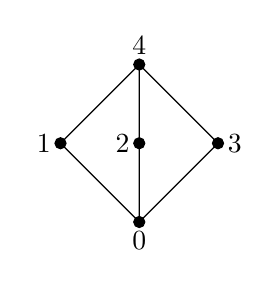
\begin{tikzpicture}
            \filldraw[black] (0,0) circle(2pt) node[above] {4} -- (-1,-1) circle(2pt) node[left] {1} -- (0, -2) circle(2pt) node[below] {0} ;
            \filldraw[black] (0,0) -- (0,-1) circle(2pt) node[left] {2} -- (0, -2) ;
            \filldraw[black] (0,0) -- (1,-1) circle(2pt) node[right] {3} -- (0, -2) ;
        \end{tikzpicture}
        \captionof{figure}{Hasse-Diagramm einer Ordnungsrelation}
    \end{minipage}

    $(\mathcal{P}(M), \cap, \cup, \emptyset, M)$ ist ein beschränkter Verband. $(\mathbb{Q}, \min, \max)$ kann hingegen nicht zu einem beschränkten Verband gemacht werden.
\end{example}

\begin{lemma}
    Jeder Verband $\mathfrak{V} = (V, \wedge, \vee)$ mit endlicher Trägermenge $V = \{v_1, \ldots, v_n\}$ kann zu einem beschränkten Verband gemacht werden.
\end{lemma}
\begin{proof}
    Sei $1 := v_1 \vee \ldots \vee v_n$, dann gilt für beliebiges $j \in \{1, \ldots, n\}$, dass $$v_j \vee 1 = v_j \vee v_1 \vee \ldots \vee v_n =  v_1 \vee \ldots \vee v_j \vee v_j \vee \ldots \vee v_n = v_1 \vee \ldots \vee v_n = 1.$$
    Analoges gilt für $0 := v_1 \wedge \ldots \wedge v_n$. Damit ist $(V, \wedge, \vee, 0, 1)$ ein beschränkter Verband. 
\end{proof}

\begin{definition}\label{def:boolsche_algebra}
    Eine Algebra $\mathfrak{A} = (A, \wedge, \vee, 0, 1, \,')$ vom Typ $\tau = (2,2,0,0,1)$ heißt \emph{Boolesche Algebra}\index{Boolesche Algebra}, wenn
    \begin{itemize}
        \item $(A, \wedge, \vee, 0, 1)$ ein beschränkter distributiver Verband ist,
        \item $\forall x \in A: x \wedge x' = 0$ und
        \item $\forall x \in A: x \vee x' = 1$
    \end{itemize}
    gilt.
\end{definition}

\begin{example}
    Für eine Menge $M$ ist $(\mathcal{P}(M), \cap, \cup, \emptyset, M, ')$ mit $'(X) := M \setminus X$ eine Boolesche Algebra.
\end{example}

\begin{remark}
    Alle Booleschen Algebren werden durch den Darstellungssatz von Stone bis auf Isomorphie beschrieben.
\end{remark}

\begin{definition}
    Seien $\mathfrak{A} = (A, (f_i^\mathfrak{A})_{i \in I}), \mathfrak{B} = (B, (f_i^\mathfrak{B})_{i \in I})$ zwei Algebren vom selben Typ $\tau = (n_i)_{i \in I}$. Eine Abbildung $\varphi: A \to B$ heißt \emph{Homomorphismus}\index{Homomorphismus}, wenn

    $$\forall i \in I \forall a_1, \ldots, a_{n_i} \in A: \varphi(f_i^\mathfrak{A}(a_1, \ldots, a_{n_i})) = f_i^\mathfrak{B}(\varphi(a_1), \ldots, \varphi(a_{n_i})). $$

    Wir schreiben dann auch $\varphi : \mathfrak{A} \to \mathfrak{B}$.

    Wenn $\varphi$ bijektiv ist, dann heißt die Funktion \emph{Isomorphismus}\index{Isomorphismus}.
    Ist $\mathfrak{A} = \mathfrak{B}$, dann heißt $\varphi$ \emph{Endomorphismus}\index{Endomorphismus}. Ein bijektiver Endomorphismus heißt \emph{Automorphismus}\index{Automorphismus}.
\end{definition}

\begin{definition}
    Zwei Algebren $\mathfrak{A} = (A, (f_i^\mathfrak{A})_{i \in I}), \mathfrak{B} = (B, (f_i^\mathfrak{B})_{i \in I})$ vom selben Typ nennen wir \emph{isomorph}\index{isomorph}, wenn es einen Isomorphismus $\varphi: \mathfrak{A} \to \mathfrak{B}$ gibt. Wir schreiben auch $\mathfrak{A} \cong \mathfrak{B}$.
\end{definition}

\begin{example}
    Sei $\mathfrak{A}$ eine Algebra. Wir definieren die Mengen \begin{align*}
        \End(\mathfrak{A}) &:= \{f: A \to A \mid f\text{ ist Endomorphismus}\} \text{ und} \\ \Aut(\mathfrak{A}) &:= \{f: A \to A \mid f\text{ ist Automorphismus}\}.
    \end{align*}

    $(\End(\mathfrak{A}), \circ, \id_A)$ ist dann ein Monoid, das \emph{Endomorphismenmonoid von $\mathfrak{A}$}\index{Endomorphismenmonoid}. Wie wir in \cref{theorem:darstellungssatz-cayley-monoid} sehen werden, ist jedes Monoid isomorph zu einem Endomorphismenmonoid.
    
    $(\Aut(\mathfrak{A}), \circ, \id_A, {}^{-1})$ ist eine Gruppe, die \emph{Automorphismengruppe von $\mathfrak{A}$}\index{Automorphismengruppe}.
\end{example}
